\chapter{Implementation}
\label{cha:implementation}

This section describes how the concept and design explained in Section 3 are implemented. The primary purpose of the implementation is a realization of proposed models that integrate into provided Staxnet system. Therefore, I give details of background information, system requirement, and implemented protocols and mechanisms in divided subsections. A description of the proposed models is given using the figures and code fragments.

\section{Background information}

The fundamental components of the system in this implementation are the Staxnet daemon and CLI application with extra data transmission functions. The given Staxnet daemon is developed by inheriting the existing design that maintains mechanisms and functions and minimizes changes. The differences of Staxnet daemon will be described in the following section. The entire applications are developed by ANSI C99 language. This implementation targets resource-constrained computers. The implementation environment is Visual Studio Code, which is Microsoft's open-source software. The build system uses GNU Autotools \cite{experimentingwithquic} that is an easy and quick opens-source tool to compile a package of source codes. Staxnet daemon applies external libraries, libevent, and libsodium \cite{Libsodium}. Libevent is used for handling the occurred asynchronous event in the system. Libsodium is a cryptographic library, which manages the overall crypto service in the system. For data transmission procedures among peers, the CLI application applies more libraries, liblsquic, and boringSSL. BoringSSL is Google designed a fork of OpenSSL \cite{BoringSSL}. LSQUIC (Lite Speed QUIC) is for QUIC and HTTP3’s open-source library \cite{lsquic}. The details of the utilized libraries will be described in the Used Techniques section. The applications are based on UNIX OS and it tested Linux of amd64, Linux of ARM processor (e.g., Raspberry pi 3 model B \cite{Raspberry}), and Apple Darwin. Unfortunately, Windows OS is not supported.

\section{Requirement}

In the previous section, we have presented two critical problems: MTU limitation and problematic protocol characteristics, to be solved in this study. Therefore, we describe what the system is required to resolve such problems. Before the Staxnet is implemented, the system should satisfy essential functional requirements.

\begin{description}
	\item[(1)]Even large data must be transmitted between peers. According to MTU limitation, this causes a traffic congestion problem when transmitting a large file. Therefore, the system should be implemented for large-size file transfers as an essential requirement. At least 5 megabytes of data should be communicated without having problems. In particular, this implementation can overcome the MTU limitation problem.
	\item[(2)]The three transport protocols that are proposed, TCP, UDP, and QUIC, implement the direct tunnel-based P2P communication model that should operate without problems. The implementation should communicate between peers using the protocols for file transmission. In addition, the CLI application allows that user can select the protocols when the file transmission procedure is initialized.
	
	\item[(3)]Cross-compiling should be supported. The goal of the system is to communicate between a personal computer and IoT device or between IoT devices. Therefore, this implementation should support the targeted resource-constrained computers and be possible to compile for the target. It needs to develop with ANSI C language because it should consider compatibility.
	
	\item[(4)]Communication must be secure. All transmittable packets among peers must be encrypted. All peers must reject to receive unencrypted packets. The system should consider malicious attacks such as packet sniffing. It is mandatory to avoid these harmful problems. Thus, the implementation should use a guaranteed reliable, robust cryptography.
	
\end{description}

The four requirements described above are essential, and they should clearly apply to the entire implemented system.

\section{Used techniques}

The implementation needs other libraries to fulfill the proposed requirements. In this section, we introduce the cryptographic and QUIC libraries.

The Staxnet daemon uses the Sodium library. It provides encryption, decryption, signatures, hashing, and more. Moreover, it supports a portable, cross-compilable, installable, and packageable fork of NaCl (Networking and Cryptography library) with a compatible API, and an extended API \cite{Libsodium}. This library is suitable to the aim of this study. The implementation should support resource-constrained computers. Also, it is implemented using ANSI C. Sodium library fulfills both requirements. Moreover, it provides what is using the most functions in the Staxnet system. Each peer must possess digital signatures (e.g., public-key, secret-key, CA). When the signatures are generated, the system uses this library. The generated signatures are used for the authentication between the peers. When a key as an identifier is stored in a DHT, the key is hashed using the SHA256 algorithm \cite{menezes2018handbook}. In the message exchange, the message is encrypted, decrypted, and authenticated. For this procedure, the system is using this library. However, a communication using QUIC protocol applies different cryptographic.

The implementation of the direct tunnel-based P2P model enables extending protocols such as QUIC protocol. QUIC improves the weakness of TCP and inherits its strengths. Because the connection establishment of QUIC is 0-RTT instead of TCP, 3-RTT, QUIC ensures less latency time. Moreover, it does not need to take one more RTT for crypto. QUIC takes advantage of transmission speed. Also, it supports congestion control and error control. When the packet loss occurs, TCP retransmits the lost packets. It causes increased traffic. QUIC can resolve this problem through congestion control and error control. It guarantees the portability of mobile devices using a connection migration. QUIC identifies a connected client through the client's specific ID. Hence, the client can maintain the connection if the client gets a new IP address; when a client moves when using a mobile network, the device's IP address is allocated. Also, if the device switches network router, it receives a newly allocated IP address. Thus, in this situation, the client should execute the connection establishment again in TCP-based network communication. According to these reasons, we consider enabling the QUIC protocol in the implementation. The QUIC protocol is still under development, and IETF is undertaking the HTTP mapping over QUIC for HTTP/3 standard. The implementation must apply other libraries to enable the QUIC protocol.

When investigating on improving transport protocols, we consider QUIC protocol to be fit for this implementation. There are several implementations using QUIC with various languages. This implementation uses the LSQUIC library, a C-based open-source implementation of QUIC and HTTP/3 functionality for servers and clients. It supports Internet-Draft versions 34, 29, and 27, and "Google" QUIC versions Q043, Q046, and Q050 \cite{lsquic}. It inherits the most features of QUIC and HTTP/3, and supports the following.

\begin{description}
	\item DPLPMTUD (Datagram Packetization Layer Path MTU Discovery) \cite{fairhurst2018packetization}
	\item ECN (Explicit Congestion Notification) \cite{draftjohanssonquicecn00}\cite{fairhurst2017benefits}
	\item Spin bits (allowing network observer to calculate a connection’s RTT)
	\item Path migration
	\item NAT rebinding
	\item Push promises
	\item TLS Key updates
\end{description}

Specifically, DPLMTUD is a discovery of transmittable maximum packet size among hosts. It is an important feature to resolve the MTU problem. This library does not provide socket communication for sending and receiving the packet. The transmission is handled by user-supplied callbacks. This library is fairly flexible to be implemented. Therefore, it is suited for making it transparent on its functionalities into an implementation. LSQUIC library require extra libraries, which are zlib for data compression \cite{zlib}, BoringSSL \cite{BoringSSL}, ls-hpack \cite{hpack}, and ls-qpack \cite{lsqpack}. The HPACK library is a compressor that eliminates redundant header fields, limits vulnerability to known security attacks, and has a bounded memory requirement for the use in constrained environments \cite{TheNetworkAccessIdentifier}. The QPACK library is a compression of the header for QUIC and HTTP/3. It was designed by inheriting the existing HPACK library. It is developed for less HOL blocking \cite{draftietfquicqpack21}. BoringSSL is designed by Google and is a fork of OpenSSL. It is currently used in Google platforms such as Chrome/Chromium, Android, and other related apps/programs.

\section{Staxnet implementations}

Staxnet project is the implementation of the MCC (Mesh Companion Component) specification. It is developed for supporting resource-constrained computer with the requirements. This project consists of the following fundamental components.

\begin{description}
	\item staxnetd
	\item staxnetctl
	\item staxnetca
	\item staxmetnode
	\item libstaxnet
	\item staxnetd.conf
\end{description}

staxnetd, which is a daemon, has the responsibility to manage a peer of the DHT network. Most communication functionalities among peers are operated through it. staxnetctl, which is a CLI interface, is used to communicate with staxnetd via Unix-domain socket. The proposed models will be implemented on it. staxnetca manages the CA and creates peer certifications. staxnetnode creates a peer identifier (node ID), which consists of public and private key pairs. libstaxnet is a collection of complete MCC node implements. All fundamental functionalities of Staxnet are implemented in the libraries. Staxnet daemon uses it for connecting to the Staxnet network. The staxnetd.conf file has a peer's information, including nodeID, certification, public key, secret key, listening to IPv4 address and port, and UNIX-socket location. The details of the implementations are given in the following sections.

\subsection{Pre-processing}

The Staxnet daemon initializes a peer with a configuration file (i.e., staxnetd.conf). 
The configuration file is mandatory to exploit the Staxnet. It consists of several entities generated by staxnetnode and staxnetca. The staxnetnode application creates the public and secret key pairs of the entities. At first, a configuration file for boot peer must be generated. When a user executes the staxnetnode application with the '-c' flag, the created random key pair is given. Both keys are base64-encoded. The public key is using for peer identifier (i.e., nodeID). The staxnetca application creates the new CA. The application is executed with the '-c' flag. It creates a random public/private key pair for the CA. Both keys are base64-encoded. The public key is written to stdout, while the private key is written by default to `./secret`. Then, the staxnetca application creates a certificate that the Staxnet daemon can use. It will include the generated nodeID and be signed by the private key pointed by default in `./secret` and sets the certificate's permissions when creating one. A comma-separated list of values is expected. Allowed values are `add`, `get`, `openchannel`, and `relay`. The configuration file is created, including the given resources. Table 4.1 shows an example of the boot configuration file.

\begin{table}[!ht]
	\small
	\centering
	\begin{tabular}{|l|l|l|l|}
		\hline
		Component & Values & Size in bytes \\
		\hline
		node ID & wcKcwHc1eDhXCrO4Y… & 32 \\
		\hline
		certificate & wcKcwHc1eDhXCrO4Y… ontAmvOug1pyiGzMk & 64 \\
		\hline
		CA’s public key & lGeYlqNeoHZISkklead… & 32 \\
		\hline
		private key & r16hExp7joLqYvysTfxt… & 32 \\
		\hline
		listen & 127.0.0.1:7777 &  \\
		\hline
		Unix-socket & ./staxnetd-boot.sock &  \\
		\hline
		mapping server & 127.0.0.1:8888 & \\
		\hline
	\end{tabular}
	\caption{Example of boot configuration file}
\end{table}

A standard peer's configuration file is created, including boot's CA and certificate. This generates random public and private key pairs and its certificate in the same method as the boot configuration generation. This configuration file includes extra values such as the boot's certificate. An example of the configuration file is shown in Table 4.2.

\begin{table}[!ht]
	\small
	\centering
	\begin{tabular}{|l|l|l|l|}
		\hline
		Component & Values & Size in bytes \\
		\hline
		node ID & GqhZqJT26Tb1ENW3Kk… & 32 \\
		\hline
		certificate & GqhZqJT26Tb1ENW3Kk … R9JJ4xfOFDtmgI & 64 \\
		\hline
		CA’s public key & lGeYlqNeoHZISkkleVn … & 32 \\
		\hline
		private key & E7sm9tbrhEoYjcd5Yel… & 32 \\
		\hline
		listen & 127.0.0.1:7778 &  \\
		\hline
		Unix-socket & ./staxnetd.sock &  \\
		\hline
		boot’s certificate & wcKcwHc1eDhXCrO4Y… ontAmvOug1pyiGzMk & 64 \\
		\hline
		mapping server & 127.0.0.1:8888 & \\
		\hline
	\end{tabular}
	\caption{Example of boot configuration file}
\end{table}

In the beginning, the initialization of the peer reads the configuration file from staxnetd. The implementation parses and verifies the given resource of the file. The including keys, which are base64-encoded, should decode into readable unsigned integer numbers as uint8. It calls a function, \textit{sodium\_base642bin( )}. After parsing and verification, it opens a socket using the peer's IPv4 address and port number. The socket is using UDP protocol for communicating among peers.

\subsection{Peer initialization}

The first step of the peer initialization is crypto library initialization. The implementation calls \textit{sodium\_init( )} method. Because a peer uses the functions provided by the Sodium library, it must be initialized as a first priority. After the initialization of the crypto library, the implementations start the creation of a new peer. It calls the \textit{staxnet\_new( )} function with a structure parameter, including network information. Initializing the peer requires three steps: (1) store a socket, (2) generate new memorial DB, and (3) manage certificates. The \textit{staxnet\_new( )} function is displayed in Listing 4.1. A staxnet structure is assigned before the steps are processed. This structure contains global data about a peer, such as the socket, database, routing table, timer, and certificates. The given socket data is added to a socket field of staxnet structure. The implementation supports the memorial DB for a peer. It does not deploy any enterprise database. The DB consists of a simple, singly linked list. A new routing table is created by \textit{routing\_node\_new( )} method. It allocates an empty binary tree and an empty bucket. Through the \textit{gettimeofday( )} method, the implementation sets the present time for the event handler. The parsed certificates must be verified. Using the \textit{crypto\_sign\_verify\_detached( )} method of the sodium library, the signature of the certificate is verified. If it is passed, the expiration of the signature is checked. The verified certificates are wrapped into the staxnet structure. When all steps are done, the initialized peer is initiated into the DHT. The event handler takes the routing table initial callback, and then the callback is executed.

\lstset{language=C} 
\begin{lstlisting}[caption=Peer initialization]
	struct staxnet*
	staxnet_new(struct staxnet_opts *opts)
	{
		struct staxnet *net = malloc(sizeof(struct staxnet));
		// We reserve 0 to indicate that the req is new.
		net->next_msgId = 1;
		net->socket = opts->socket;
		net->fromlen = sizeof(net->from);
		net->db = db_new();
		// Init routing.
		net->routing = routing_node_new();
		net->routing->isNear = true;
		// Init time.
		if (gettimeofday(&net->tv, NULL) == -1) {
			WARN("gettimeofday failed: %s", strerror(errno));
			return NULL;
		}
		// Verify signature of certificate.
		if (staxnet_cert_verify(&opts->cert, opts->ca_pk) != 0) {
			WARN("failed to verify node cetificate signature");
			return NULL;
		}
		// Check if certificate is still valid.
		cert_tv.tv_sec = opts->cert.timestamp;
		cert_tv.tv_usec = 0;
		if (!timercmp(&net->tv, &cert_tv, <)) {
			WARN("node certificate expired");
			return NULL;
		}
		// Save certificate.
		memcpy(&net->cert, &opts->cert, sizeof(struct staxnet_cert));
		memcpy(net->sk, opts->node_sk, STAXNET_NODE_SECRETKEY_SIZE);
		memcpy(net->ca_pk, opts->ca_pk, STAXNET_CA_PUBLICKEY_SIZE);
		// Init neighbors.
		neighbors_init(&net->n);
		timeradd(&net->tv, &timeout_neighbors, &net->n.ev.timeout);
		event_insert(&net->evq, &net->n.ev);
		
		return net;
	}
	
\end{lstlisting}

\subsection{Mapping address}

The legacy Staxnet system has no mapping service. Therefore, the regular peer accesses the boot peer using the configuration file that contains the boot peer's IP address and port. This mapping server is an extra deployed service. We design it to avoid exposing the address and to give the flexibility in establishing the boot peer with a different address dynamically. Moreover, the address data will be encoded in the DB. Also, it is used to get a requested peer's address in the direct tunnel-based P2P model. Because of this service, the system complexity is increased. All peers must first communicate with this server. Furthermore, when communication is disturbed, it becomes a big problem. This should be improved to overcome future work.

The architecture is simple and it uses the UDP protocol to communicate. Figure 4.1 shows the procedure of the mapping server. There are three procedures for the mapping address.

\begin{figure}[!ht]
	\centering
	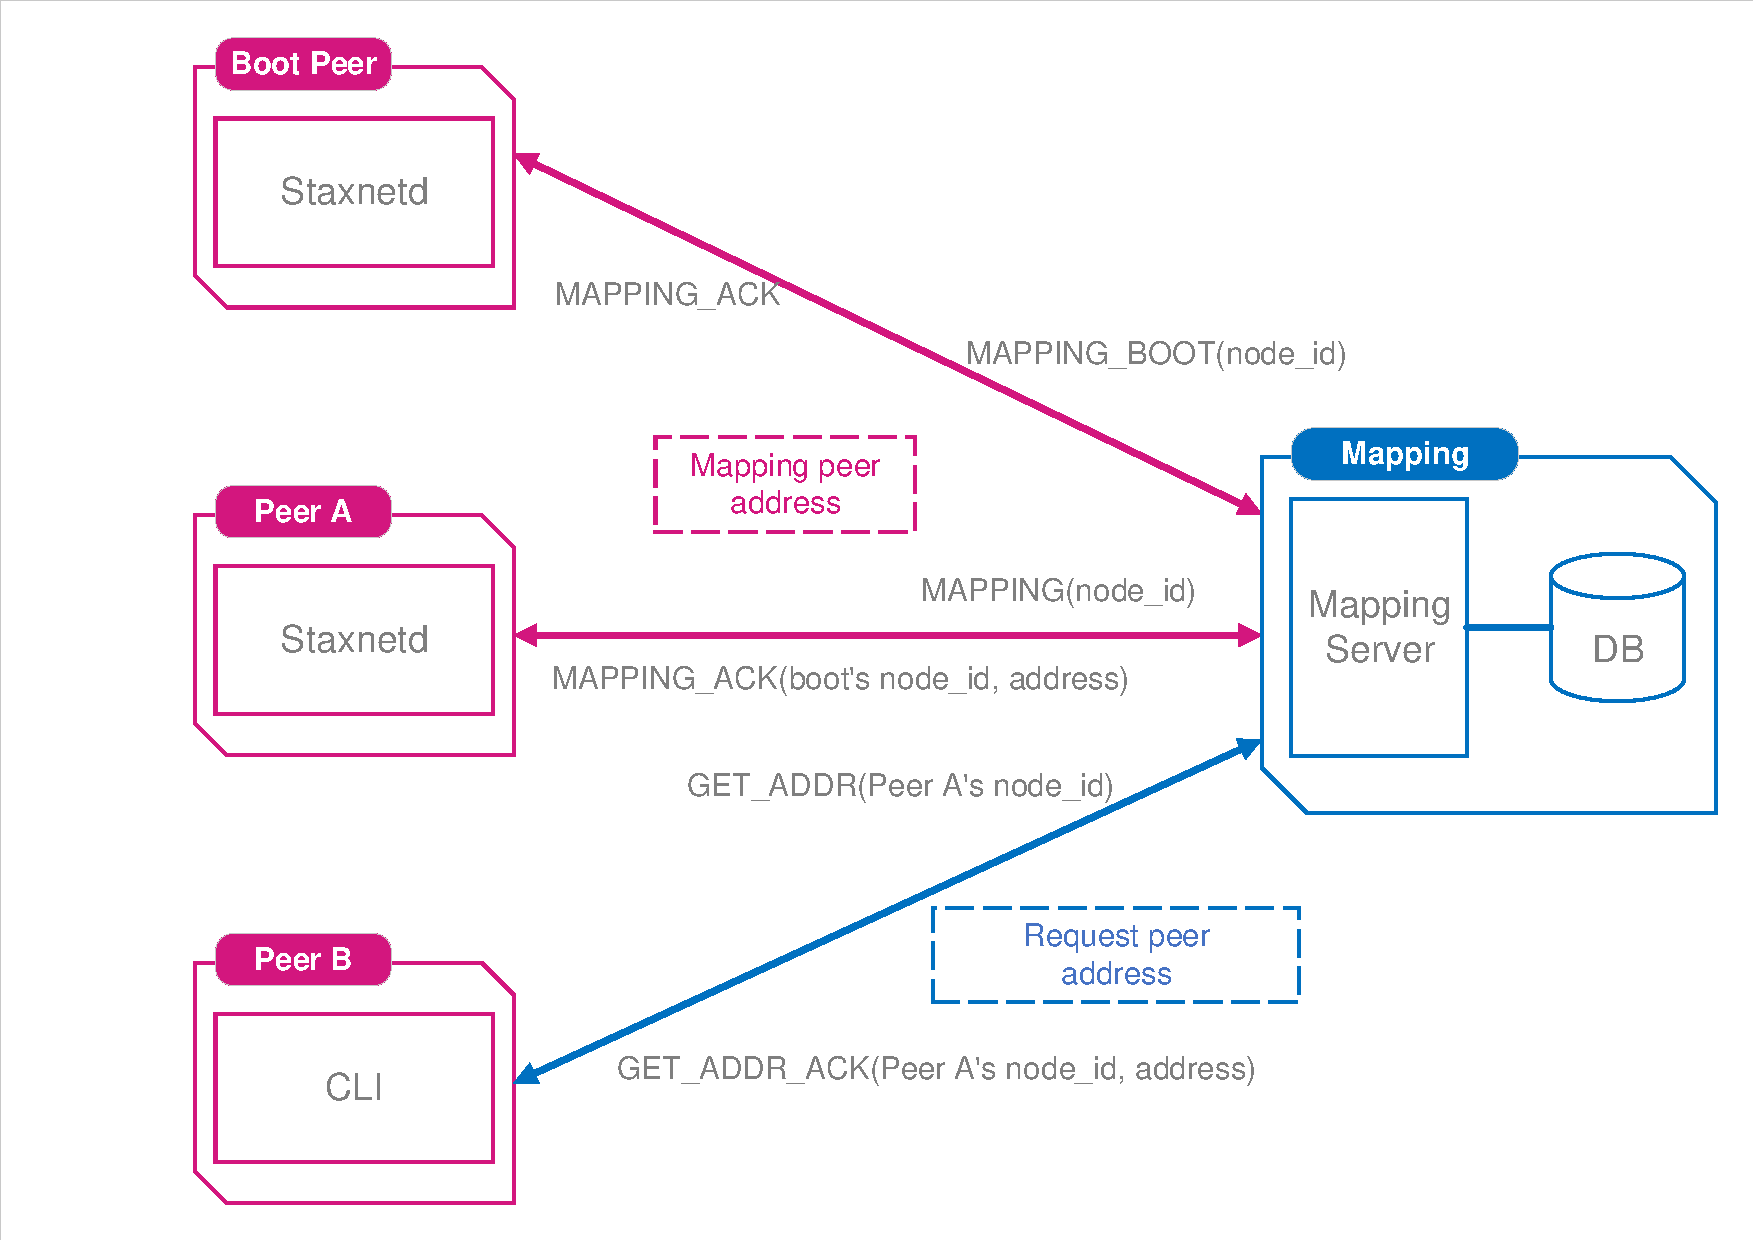
\includegraphics[width=0.5\textwidth]{images/fig_4_1.pdf}\\
	\caption{Three procedures of the mapping address}
	\label{fig:mapping}
\end{figure}

\begin{description}
	\item[Boot peer] This procedure is between the boot peer and the mapping server. The boot peer sends a message with the \textit{'MAPPING\_BOOT' }flag, including its unique \textit{node\_id}. Before the request, the payload will be encrypted by the XChaCha20-Poly1305. When the mapping server received the message, the chipper message will be decrypted by the shared secret key. It is stored in the mapping server's DB. In this server, it uses the memorial DB the same as the Staxnet daemon. The server responds to the message with the \textit{'MAPPING\_ACK'} flag.

	\item[Regular peer] Before this procedure begins, the boot peer must be mapped. The peer sends the message, \textit{'MAPPING'} flag. This method is the same as boot peer. The mapping server stores the received \textit{node\_id} and address in the DB, and then it looks up the boot peer's information. The server responds to the message with the \textit{'MAPPING\_ACK'} flag, including the boot peer's \textit{node\_id} and IPv4 IP address. The responded message is also encrypted. The daemon must decrypt it to use.

	\item[CLI application] In the direct tunnel-based P2P model, the CLI application as a client gets a target peer's \textit{node\_id} from the MCC. The CLI should know the target peer's address to make a tunnel. It requests to the mapping server the target's address. Therefore, it sends a message with \textit{'GET\_ADDR'} including given \textit{node\_id}. The message is also encrypted. The mapping server looks up the peer information in the DB using the received \textit{node\_id}. If the peer exists, the data, which are \textit{node\_id} and IPv4 address pairs, is sent back to the CLI application. The CLI application begins to make a tunnel using the received target's peer information.
\end{description}

\subsection{Ping to peers}

The P2P network system gives peers great autonomy. Each peer can dynamically participate in the P2P network or leave it easily. It is called churn \cite{medrano2013effect}. Churn can induce grave situations on DHT-based P2P networks. The network has set the rules to locate the peer. In Kademlia DHT, it follows the distance between the peers, that the distance is calculated by XOR metric. The location of the participated peer is determined on the network. The network topology is created by this logic. Suppose that a peer left from the network and the topology does not recognize this situation. The lookup service may not be possible to retrieve the correct value. It affects the reducing performance of Kademlia DHT. Therefore, the topology must be updated \cite{bustamante2004friendships}\cite{stutzbach2006understanding}\cite{stutzbach2006understanding}. 

The Staxnet daemon offers a ping service to check churn or to do a handshake. When the initialized peer processed the mapping address, the peer sends the ping message to the boot peer with the 'PING' flag. The message includes the session key for the crypto handshake. The peer calls the \textit{staxnet\_pingByAddr( ) method}. Listing 4.2 illustrates the sending ping to the boot peer.

\lstset{language=C} 
\begin{lstlisting}[caption=Sending ping to the boot peer]
	int
	staxnet_pingByAddr(struct staxnet *net, struct staxnet_addr *addr, staxnet_cb cb)
	{
		int err;
		struct ping *p = malloc(sizeof(struct ping));
		
		//DEBUG("called");
		
		p->cb = cb;
		p->ctx = NULL;
		// Message payload init.
		req_init(net, &p->req, PING, ping_loop, p); 
		p->req.msg.len = 0;
		err = send_request(net, &p->req, (struct sockaddr*)(&addr->sa),
		sizeof(struct sockaddr_in), addr->cert.nodeID);
		if (err != 0) {
			return err;
		}
		
		return 0;
	}
	
	
\end{lstlisting}

The implementation assigns a ping structure. It initializes the callback, \textit{'ping\_loop'}, using the \textit{req\_init( )} method. The payload is empty because the ping message does not need to involve any message, and then, it is sent to the boot peer with the session key. When the waiting boot peer received the message, it is handled by the \textit{handle\_ping( )} method. The boot peer responds to the message with \textit{'PING\_ACK'}; this message will be encrypted using the server session key, which is made using the received peer's public key. If the peer received the message from the boot peer and could decrypt the given payload, the ping procedure for a handshake is successful. Listing 4.3 shows the \textit{handle\_ping( )} method.

\lstset{language=C} 
\begin{lstlisting}[caption=The handle\_ping( ) method]
static void
handle_ping(struct staxnet *net)
{
	// msg->header.reqID is already set.
	net->msg.header.type = PING_ACK;
	staxnet_cert_pack(&net->cert, net->msg.header.cert);
	net->msg.len = 0; // Ack has no payload.
	//DEBUG("net->tx : %ld",net->tx);
	msg_wire_init(&net->mw, &net->msg, net->tx);
	send_wire(net, &net->mw, &net->from, net->fromlen);
}

	
\end{lstlisting}

The second purpose of the ping service is to check churn. When a peer is in idle time, it sends a ping message to neighbor peers in a bucket. This procedure is initialized in the event handler when the peer is created. It gets the neighbor peer list by the \textit{shortlist\_dequeue( )} method. Until the next peer does not exist, it proceeds the ping service. This algorithm is explained in Listing 4.4.

\lstset{language=C} 
\begin{lstlisting}[caption=The neighbors\_loop( ) method]
	static void
	neighbors_loop(struct staxnet *net, struct req *req, void *ctx)
	{
		struct neighbors *n = ctx;
		struct info *peer = shortlist_dequeue(n->sl);
		
		if (req->retry == MAX_RETRY)
		DEBUG("req timed out; trying next");
		
		if (peer == NULL) {
			shortlist_free(n->sl);
			
			timeradd(&net->tv, &timeout_neighbors, &n->ev.timeout);
			event_insert(&net->evq, &n->ev);
			
			return;
		}
		
		DEBUG("Neighbors PING -> " ID_F_ARG, ID_ARG(peer->cert.nodeID));
		
		if (send_request(net, req, &peer->sa, peer->salen, peer->cert.nodeID) != 0) {
			WARN("Failed to send request to peer; try next one");
			neighbors_loop(net, req, ctx);
		}
	}
	
\end{lstlisting}
The network topology can update the state of participated peers via the ping service. Therefore Staxnet can keep maintenance of DHT performance.

\subsection{Routing table}

Kademlia routing table consists of a binary tree; its leaves are \textit{k}-buckets. The peer belongs to the \textit{k}-bucket. The peer is located in the binary tree using each bit of the peer's identifier as \textit{node\_id}. The \textit{node\_id} is \textit{160}-bit ID space. The systems set a maximal bucket range as twenty. The \textit{k}-buckets cover all \textit{160}-bit apace with no overlap \cite{bibid}[9]. The methodology of the Kademlia routing table is explained in Section 2.4.1. 
When the system updates the routing table, it calls the \textit{routing\_update( )} function. In the function, the system occurs in finding a node, allocating a new node, and updating a bucket. We give the explanation using Listing 4.5 to help with the understating.

\lstset{language=C} 
\begin{lstlisting}[caption=The procedure to deal with input data]
	void
	routing_update(struct staxnet *net, struct info *info)
	{
		struct routing_node *n = net->routing;
		
		// Find correct leaf node.
		for (int i=0; i < 19; i++) {
			for (int j=0; j < 7; j++) {
				// Leaf nodes, have both zero and one set to NULL.
				if (n->zero == NULL) {
					// If bucket has space, we update it.
					if (bucket_update(n->bucket, info) == 0)
					return;
					
					// Bucket has no space and is not near. In this case
					// we ping the LRU entry.
					if (!n->isNear) {
						// TODO Implement this case.
						return;
					}
					
					// Alloc nodes.
					n->one = routing_node_new();
					n->zero = routing_node_new();
					
					// Set isNear.
					n->isNear = false;
					if (IS_ID_BIT_SET(net->cert.nodeID, i, j)) {
						n->one->isNear = true;
					} else {
						n->zero->isNear = true;
					}
					
					// Re-insert bucket entries (infos) into new buckets.
					struct bucket_entry *next, *e = n->bucket->head;
					do {
						next = e->next;
						if (IS_ID_BIT_SET(e->info->cert.nodeID, i, j)) {
							bucket_insertEntry(n->one->bucket, e);
						} 
	
					} else {
						bucket_insertEntry(n->zero->bucket, e);
					}
					e = next;
					} while(next != NULL);

					// Free bucket.
					free(n->bucket);
					n->bucket = NULL;
				}

				if (IS_ID_BIT_SET(info->cert.nodeID, i, j)) {
					n = n->one;
				} else {
					n = n->zero;
				}
			}
		}
	}


\end{lstlisting}

It finds the correct leaf node using the for a loop. When the leaf nodes, which are zero and one, are set to null, they are empty. It attempts to update the bucket when the bucket has space, and then, the routing update is done. Therefore, this function will be terminated. Otherwise, when the bucket is full, it allocates new nodes and a new bucket. The routing node configures near nodes. The list of the bucket will be updated again. The leaf nodes are not empty, and the bit set of the given \textit{node\_id} exists, and the routing node is updated according to the bit set of the \textit{node\_id}. 

The system using this implementation of the Kademlia routing table supports the update of a new peer service and the retrieval service.

\subsection{Connection to the CLI application}

The Staxnet daemon is used for managing full services relevant to a peer in the network. This interacts with a user-interface, the CLI application. A user orders the commends using the CLI to the Staxnet daemon. This interface is provided by staxnetctl. Both applications are interconnected via a connection-oriented Unix domain socket as TCP. They establish a connection using the file system as their address namespace; CLI's address namespace is specified in the configuration file. The daemon is capable of maximizing ten connections of the CLI application. It manages the connections using the \textit{select( )} function, providing ready for reading, ready for writing, ready for waiting, and return an error functionalities. Listing 4.6 shows the connection establishment.

\lstset{language=C} 
\begin{lstlisting}[caption=The connection establishment]
FD_ZERO(&socks);
FD_ZERO(&wsocks);
FD_SET(sa_un, &socks);
highsock = sa_un;

for (i = 0; i < MAX_CLI_CONN; i++) {
	if (conns[i] != 0) {
		FD_SET(conns[i], &socks);
		if (conns[i] > highsock)
		highsock = conns[i];
	}
	if (reqs[i] != NULL && reqs[i]->state == REPLY) {
		FD_SET(reqs[i]->sock, &wsocks);
	}
}
staxnet_calcTimeout(net, &timeout);
// Select.
nsocks = select(highsock+1, &socks, &wsocks, NULL, &timeout);
if (nsocks == -1) {
	perror("select");
	exit(EXIT_FAILURE);
} 
// Check for new connections.
if (FD_ISSET(sa_un, &socks)) {
	conn = accept(sa_un, NULL, NULL);
	if (conn == -1) {
		perror("accept");
		continue;
	}
	
	for (i=0; i < MAX_CLI_CONN; i++) {
		if (conns[i] == 0) {
			// We got room for the new connection, make it nonblocking then save it.
			fcntl_opts = fcntl(conn, F_GETFL);
			if (fcntl_opts == -1) {
				perror("fcntl(F_GETFL)");
				exit(EXIT_FAILURE);
			}
			err = fcntl(conn, F_SETFL, fcntl_opts | O_NONBLOCK);
			if (err == -1) {
				perror("fcntl(F_SETFL)");
				exit(EXIT_FAILURE);
			}
			conns[i] = conn;
			break;
		}
	}
	if (i == MAX_CLI_CONN) {
		fprintf(stderr, "Too many cli connections; dropping new one");
		close(conn);
	}
}


\end{lstlisting}

When the daemon gets a new connection request from the CLI application, the system calls \textit{accept( )} function, and it returns a new file descriptor. The connection in this system is based on non-blocking communication. The created file descriptor will be set as non-blocking using the \textit{fcntl( )} method with the \textit{F\_GETFL} flag, and then it will be stored in the file descriptor array.
The system provides the daemon to monitor a maximum of ten CLI; the daemon is waiting in the idle time until the state of file descriptors has changed. When the file descriptor's state has changed to read or write, the system checks for input data from connected CLI clients using the \textit{FD\_ISSET( )} method. In the case of the write, the daemon reply to the CLI clients. In case of the read, get a message from the client. After the transmission is completed, the file descriptor will be initialized. The received message is handled in the \textit{handle\_req( )} function. This procedure to deal with input data is explained in Listing 4.7.

\lstset{language=C} 
\begin{lstlisting}[caption=The procedure to deal with input data]
// Check for input data from conntected cli clients.
for (i=0; i < MAX_CLI_CONN; i++) {
	if (FD_ISSET(conns[i], &wsocks)) {
		reply(reqs[i]);
	}
	if (FD_ISSET(conns[i], &socks)) {
		if (reqs[i] != NULL && (reqs[i]->state == REPLY || reqs[i]->state == PENDING)) {
			fprintf(stderr, "Request or response still pending for this socket, read reply before sending new requests\n");
			continue;
		}
		
		if (reqs[i] == NULL) {
			reqs[i] = malloc(sizeof(struct req));
			reqs[i]->sock = conns[i];
			reqs[i]->len = 0;
			reqs[i]->state = READ;
			reqs[i]->i = i;
		}
		rc = 0;
		do {
			rc = read(conns[i], ((char*)(&reqs[i]->msg))+reqs[i]->len,
			sizeof(struct msg)-reqs[i]->len);
			if (rc <= 0)
			break;
			reqs[i]->len += rc;
		} while (reqs[i]->len != sizeof(struct msg));
		// Check for error codes.
		if (rc == -1) {
			if (errno != EWOULDBLOCK) {
				perror("read");
				exit(EXIT_FAILURE);
			}
		} else if (rc == 0) {
			close(conns[i]);
			conns[i] = 0;
			free(reqs[i]);
			reqs[i] = NULL;
			break;
		}
		// Check if message is complete.
		if (reqs[i]->len == sizeof(struct msg)) {
			reqs[i]->state = PENDING;
			reqs[i]->len = 0;
			
			handle_req(net, reqs[i]);
		}
	}
}
	
\end{lstlisting}

\subsection{Add key-value pairs procedure}

If the CLI application attempts to insert a new key-value pair, the daemon calls the \textit{staxnet\_add( )} function. The system prepares to add them and transmit them to other peers through this function. Listing 4.8 is shown as the procedure to add key-value pairs. The given key-value pairs are decrypted through crypto preprocessing. The given key is hashed to add in the routing table, and then it sets to an allocated add structure. The key-value pair is stored in the memorial DB. When the preparation is done, this procedure will be registered in the event handler. The event handler will execute data transmission to other peers in the bucket. When the update is completed, the daemon sends back the message to the CLI application with the \textit{MSG\_ADD\_ACK} flag.

\lstset{language=C} 
\begin{lstlisting}[caption=The procedure add key-value pairs]
int
staxnet_add(struct staxnet *net, char *key, size_t keylen, char *val, size_t vallen, 
staxnet_cb cb, void *ctx)
{
	struct add *a;
	struct db_kv *kv;
	struct ev_republish *e;
	uint8_t keyID[STAXNET_ID_LENGTH];
	
	// Hash key.
	if (id_hash(keyID, key, keylen) != 0)
	return STAXNET_ERR_HASH;
	
	a = add_new(keyID, val, vallen, cb, ctx);
	// Add to DB and register republish event.
	kv = db_add(net->db, keyID, val, vallen);
	if (kv != NULL) {
		e = malloc(sizeof(struct ev_republish));
		
		e->kv = kv;
		e->net = net;
		
		// Init event.
		e->ev.cb = ev_republish;
		e->ev.ctx = e;
		timeradd(&net->tv, &timeout_kv_republish, &e->ev.timeout);
		
		// Register event.
		event_insert(&net->evq, &e->ev);
	} 
	
	return lookup_start(net, keyID, add_start, a);
}

	
\end{lstlisting}

\subsection{Get value procedure}

The DHT system stores data as a key-value pair; the key is pointing to the corresponding values. The key-value paired data search retrieves the required values using the associated key. Hence CLI application should deliver the associated key into the daemon through the user-interface. When the CLI executes the lookup service, a user inputs an argument as the key through CLI.

CLI application sends the message to the daemon with the \textit{'MSG\_GET'} flag. The daemon that received the msg via the UNIX domain socket checks the including the flag, then calls the \textit{staxnet\_get( )} method. Listing 4.9 shows the code fragment that retrieves the value using the received key. The given key should be processed to the hashed key; all keys are hashed in the system. The hashed key, the callback function, and the peer structure are assigned to the allocated get structure, which is used for the getting value method. If the daemon finds the relevant value lists with the key in the DB of its system, data of the value are extracted from the value list and are assigned into the getting structure. The daemon calls the \textit{lookup\_start( )} method to retrieve the key-value paired in other peers.

\lstset{language=C} 
\begin{lstlisting}[caption=The procedure to get the value]
	Int staxnet_get(struct staxnet *net, char *key, size_t keylen, staxnet_cb cb, void *ctx)
	{
		struct get *g;
		struct db_valHead *h;
		struct db_valEntry *v;
		struct staxnet_val *sv;
		uint8_t keyID[STAXNET_ID_LENGTH];
		// Hash key.
		if (id_hash(keyID, key, keylen) != 0)
		return STAXNET_ERR_HASH;
		g = get_new(keyID, cb, ctx);
		// Query local DB for KV-pairs.
		h = db_get_head(net->db, keyID);
		if (h != NULL) {
			SLIST_FOREACH(v, h, entries) {
				sv = malloc(sizeof(struct staxnet_val));
				// Copy.
				memcpy(sv->data, v->val, v->len);
				sv->len = v->len;
				// Insert at beginning.
				sv->next = g->res.head;
				g->res.head = sv;
				// Increment result length.
				g->res.len++;
			}
		}
		// Query staxnet for KV-pairs.
		return lookup_start(net, keyID, get_start, g);
	}
	
	
	
\end{lstlisting}

\lstset{language=C} 
\begin{lstlisting}[caption=The method of compare values]
for (v=g->res.head; v != NULL; v = v->next) {
		cntl++;
		//  continue;
		if ((memcmp(v->data, val, v->len) == 0) && v->next == NULL)
		{
			DEBUG("break");
			free(val);
			break;
		}
	}
	// If val does exist continue.
	if (v != NULL)
		break;
	// Link them together.
	v = malloc(sizeof(struct staxnet_val));
	v->next = g->res.head;
	g->res.head = v;
	// Inc lenght.
	g->res.len++; 
	// Copy data.
	v->len = vallen;
	memcpy(v->data, val, vallen);
}
	
\end{lstlisting}

When the matched key-value paired is found in another peer, it compares to the values from the source peer if the source peer includes the values from their DB. If the newly found values are longer than old values, the new one will store in the get structure, and then it keeps searching in another peer; the values consist of the set of linked lists. Therefore, the length of the values means that longer lists have more data. Listing 4.10 shows the method of compare values.

The lookup service keeps updating the value list until all peers are visited. The updated result will be processed using the callback function. In the callback function, the found data sends back to the CLI application.

\section{All peers propagation model}
In the previous section, we explain the fundamental features of Staxnet implementations. The purpose of this study is to find a large data transmission using the basic Staxnet daemon and CLI application and to improve the transmission. This model is a control model used for comparison with the direct tunnel-based P2P model. 

We designed the CLI application to attempt a large file transmission. The legacy CLI application gets a specific key and value through the user-interface. However, the CLI of this model gets the transmittable file. The file name is a key, and the file is a value marked as key-value pairs. We explain how the give key and value are stored in the DB. The memorial DB in the system uses the singly linked list. The key is a head of the list and the values that are split into 1316 bytes each become sequence linked lists.
The size of value is restricted to 1316 bytes because the size of a packet follows the MTU size, and the header space is restricted to 184 bytes. We give an explanation with Figure 4.2 to help the understating. After the key-value pair is added in the peer, the daemon propagates to peers in its bucket through the routing table update service. If another peer wants to download this key-value pair, the peer looks up this key-value paired using the key as the file name, and then it is possible to download this file without any request to the source peer. This model is a simple data transmission implementation.

\begin{figure}[!ht]
	\centering
	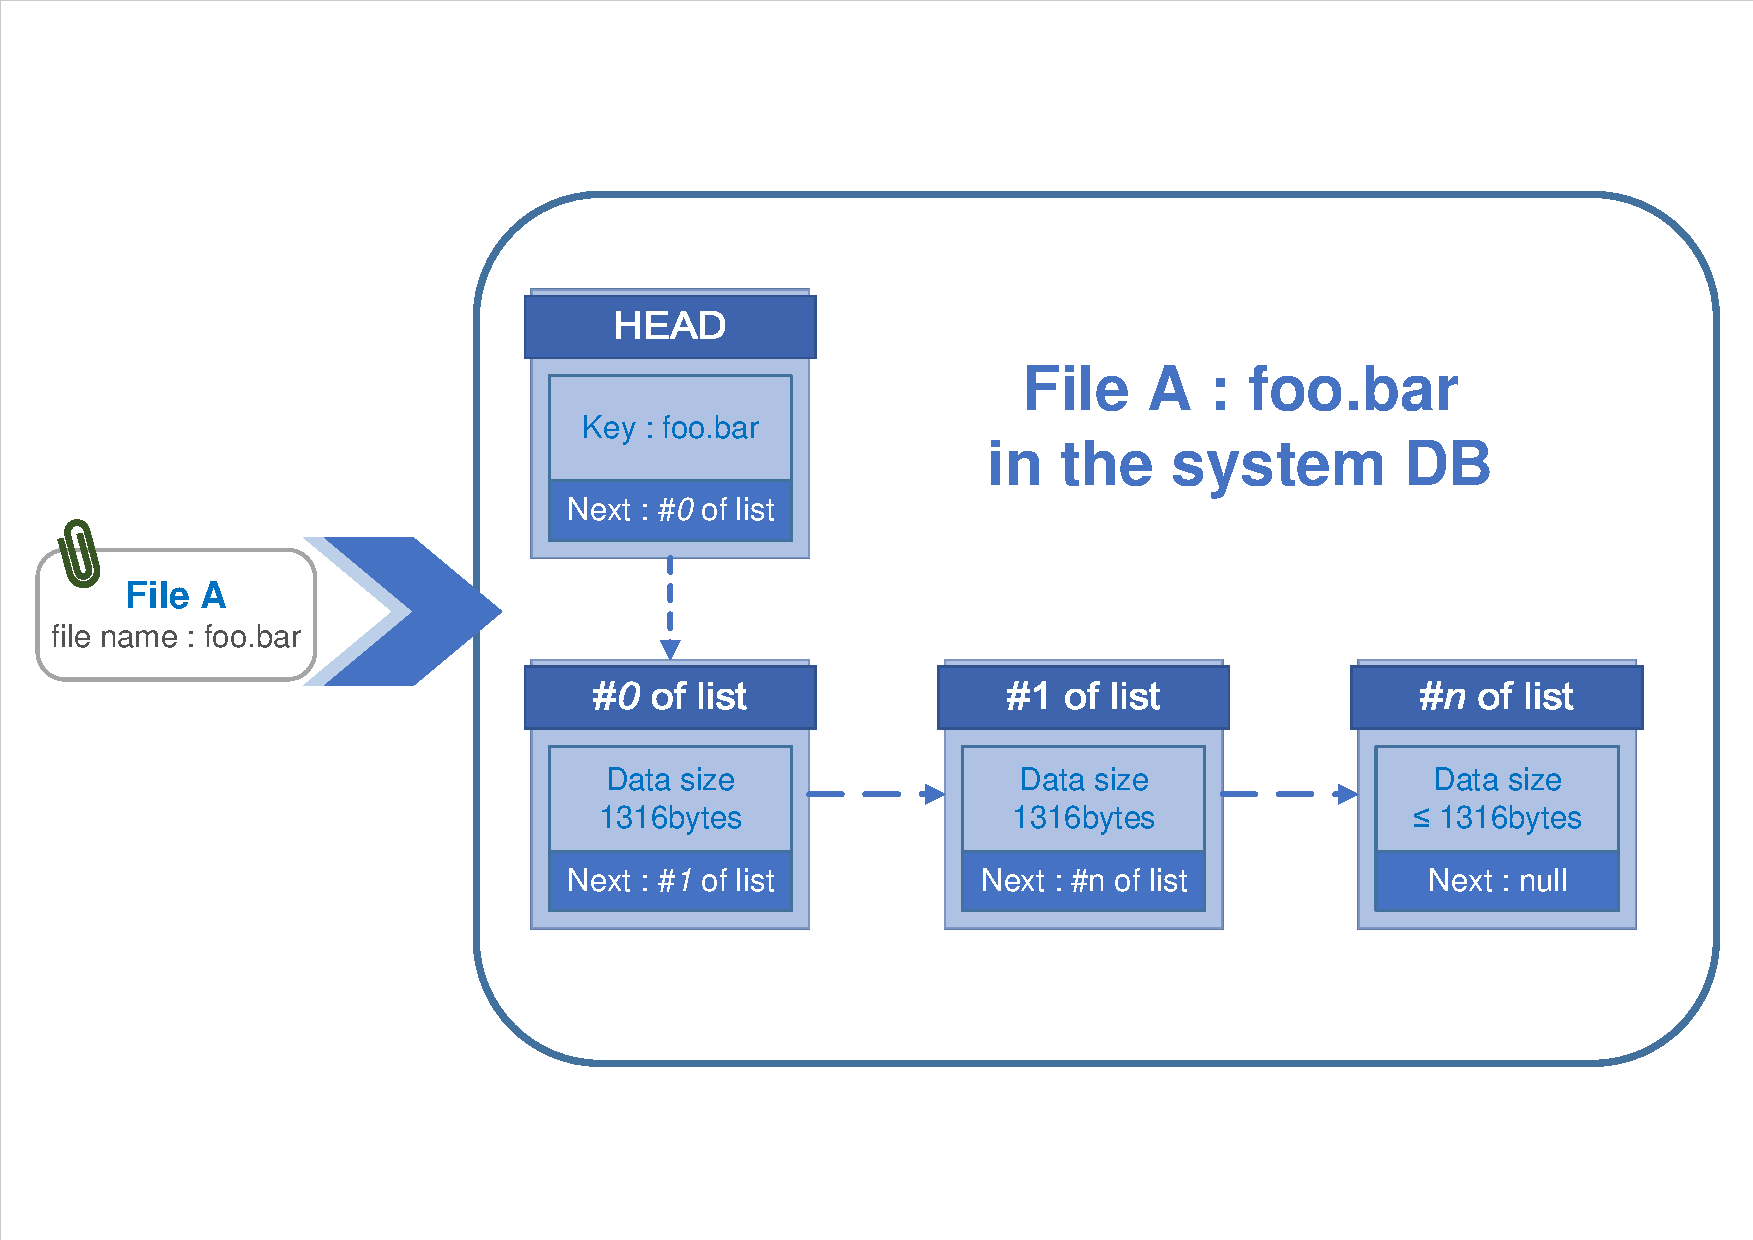
\includegraphics[width=0.5\textwidth]{images/fig_4_2.pdf}\\
	\caption{The large file transformation to the singly linked in DB}
	\label{fig:DB}
\end{figure}

\section{Direct tunnel-based Peer-to-Peer model}

The direct tunnel-based P2P model is designed to reduce the overload of the DHT network and to increase the lookup speed using a small size of key-value paired data. All peers propagate model sets that the key-value pairs on the file name and data of the file. However, this model pairs the file name and peer's node id as key-value pair. The CLI application of this model reads a given file from the user-interface, and then it sends a message to the daemon including only file name with \textit{'MSG\_ADD'} flag; this client possesses the file and becomes a sender. The daemon begins to execute the added service. It sets the key-value paired using the received file name as key and own \textit{node\_id} as value. The daemon exploits the routing table update service in order to distribute. When another peer, it refers to peer B, desires to download the file, peer B sends its daemon a request message including file name with the \textit{'MSG\_GET'} flag. The daemon retrieves using the received key as file name from the Kademlia DHT network. If the key-value pair exists, the daemon returns the found key-value paired to the CLI application. Peer B can request to the peer possessed the particular file and becomes a receiver. In this implementation procedure, the system uses the peer's node id as a value because the Staxnet daemon has mapped the peer's address using the own node id in the mapping server. Peer B requests the target's address information to the mapping server. It sends a request message including the target's node id, and then, the mapping server returns the matched IPv4 address and port number if the node id is already registered. Both peers are ready to make a direct transmittable tunnel between them.

\begin{figure}[!ht]
	\centering
	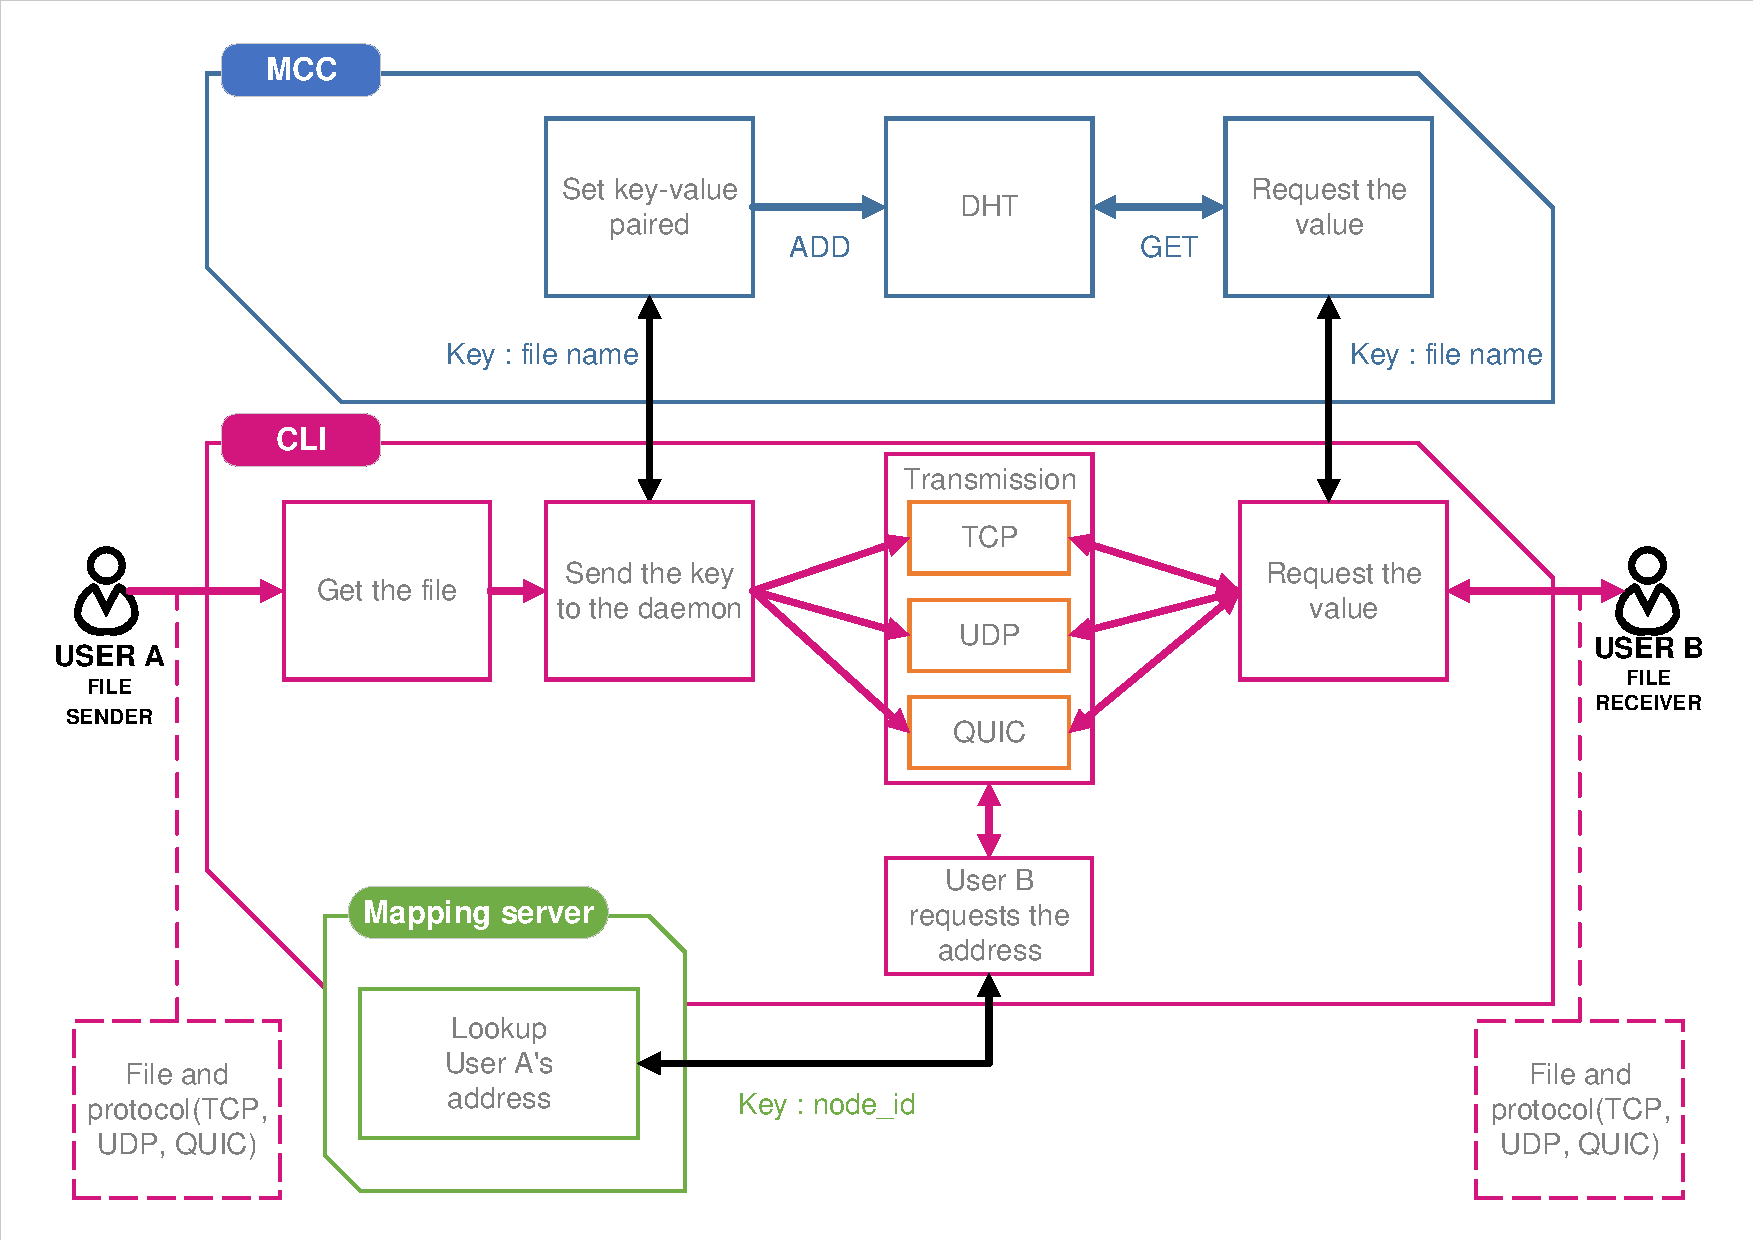
\includegraphics[width=0.5\textwidth]{images/fig_4_3.pdf}\\
	\caption{Overview of the implementation}
	\label{fig:implementation}
\end{figure}

The CLI application must get two arguments file namespace and the name of transport protocols such as TCP, UDP, and QUIC through the user-interface; it is the mandatory selection. Both peers must use the same protocol to make a new connection. The peer, which possesses the file, is ready to transmit a file after it received the message from the daemon that the key-value paired is added. Peer B request the target peer to make a tunnel. If the tunnel is made, the file transmission begins. Figure 4.3 illustrates the overview of the implementation.

\subsection{Common pre-processing}

The CLI application executes the transmission service to transfer or receive data. It calls for different methods according to the selected protocol. Each transmission method has different implementations. However, at the first step of the transmission, the implementations prepare the common pre-processing to send or receive the data. The transmission divides into the server and the client. The communication between the peers uses the secure method the same as the DHT peer communication in the Staxnet using the sodium library. This implementation reuses the config file. It parses from the existing config file; IPv4 address, certificates, and the mapping server address are extracted to reuse them. Using the IPv4 address, the implementation opens the socket, and then it initializes the sodium library. The peer is initialized using the opened socket and parsed certificates. At the server-side, the peer as the server starts waiting for a new request message. On the other side, as the client, the peer requests the mapping server to get the server’s address. It sends the request message, including the given node id from the daemon. When the response arrives, it can attempt to communicate with the server peer. TCP and QUIC transmissions should make a new connection for getting the address because the mapping server is working using the UDP protocol. TCP and UDP transmission require the crypto handshake because all packets must be encrypted in the transmission. The implementation of the client calls the \textit{ping\_to\_server( )} method, which sends to the server the ping message. The client and server exchange the certificates and make their session key. The QUIC transmission uses different crypto. Therefore, it has a different implementation in this step. It will be explained in the QUIC transmission section. After the crypto handshake is established, file sharing can begin.

\lstset{language=C} 
\begin{lstlisting}[caption=The TCP file transmission]
while(true)
{
	bzero(file_buf, MSG_PAYLOAD_SIZE);
	bzero(net->msg.payload, MSG_PAYLOAD_SIZE);
	fpsize = fread(file_buf, 1, MSG_PAYLOAD_SIZE, fp);
	memcpy(net->msg.payload, file_buf, fpsize);
	net->msg.len = fpsize;
	//usleep(200);
	if (reply_tcp(net, client_info) != 0)
	{
		perror("failed to send to the client");
		exit(EXIT_FAILURE);
	}
	if(fpsize == 0)
	break;
}

\end{lstlisting}

\subsection{TCP transmission}

Before the implementation receives the ping message from the client peer, the server peer reads the file to transfer. After the crypto handshake, the client peer sends the request message with the \textit{‘GET\_DATA’} flag. The server peer transmits data per 1316 bytes; this implementation follows the MTU limitation. It continues transferring packets until the last packet is transferred. Listing 4.11 shows the TCP file transmission.

Because each packet must be encrypted to send, the server peer uses the \textit{reply\_tcp( )} function; this function provides the encryption and transferring service. The payload is encrypted by the \textit{msg\_wire\_init( )} method. This method is used in entire Staxnet implementations. This implementation in Listing 4.12 is shown as the encrypt procedure of the payload. The implementation encrypts the payload using the generated session key; the encryption uses the XChaCha20-Poly1305 algorithm. It is provided by the sodium library.
When all packets are sent to the client peer, the transmission is terminated.

\subsection{UDP transmission}

The UDP transmission is the same as the TCP transmission. However, it is simpler than TCP because the UDP protocol is the connectionless transport protocol. It does not need a connection establishment procedure. When the server peer opens a socket, the client peer is able to connect directly. The other parts of the implementation proceed the same as TCP. When the server peer sends the last packet, this implementation cannot catch which packet is the last. Therefore, it should send the message with the specific flag, and then the client can recognize the end of the transmission when the message with the flag, the transmission is terminated.

In this section, we explain payload decryption. Listing 4.13 is shown as the decrypt procedure of the payload. When the client peer receives the message, it also generates the session key using shared keys using the \textit{crypto\_kx\_server\_session\_keys( )} method; the sodium library provides it. It calls the \textit{msg\_wire\_get\_payload( )} function with the received payload and the generated key. The \textit{crypto\_aead\_xchacha20poly1305\_ietf\_decrypt( )} function decrypts the payload. It verifies the chipper payload is encrypted by the XChaCha20-Poly1305 algorithm and decrypts. We describe the implementations of the TCP and UDP transmission. The following section gives an explanation of the QUIC transmission.

\lstset{language=C} 
\begin{lstlisting}[caption=The implementation of the payload decryption]
int
msg_wire_get_payload(struct msg_wire *w, struct msg *msg, const uint8_t *rx)
{
	int err;
	struct msg_wire_ad ad = {
		.type = msg->header.type,
		.reqID = msg->header.reqID
	};
	err = crypto_aead_xchacha20poly1305_ietf_decrypt(msg->payload, &msg->len,
	NULL, w->data+MSG_HEADER_SIZE, w->len-MSG_HEADER_SIZE, (uint8_t*)&ad,
	sizeof(struct msg_wire_ad), msg->header.nonce, rx);
	return err;
}
	
\end{lstlisting}

\subsection{QUIC transmission}

QUIC transmission adopts the LSQUIC library. Hence, this implementation is quite different from other implementations of the transmission. Moreover, it is designed for HTTP/3 support. We consider that it requires different cryptography. Inevitably, only this implementation uses an extra X.509 certificate for TLS/SSL. The system should prepare the certificate and input the certificate namespace in the configuration file. In the pre-processing step, the QUIC transmission is parsing the certificates. The client peer uses the existing certificates using the sodium library and this x.509 certificate because it communicates with the mapping server to look up the sever peer’s address. For this reason, the client-side transmission uses existing implementations of other transmissions.

At first, the QUIC transmission sets up the QUIC engine. The implementation initializes the QUIC engine, listen-address, and callback functions. This implementation calls the method using a specified callback list. The next step is the source file that inserts into the TAILQ; this LSQUIC implementation manages the connection contexts using the TAILQ. Then, the parsed certificate must be verified. After all steps of the initialization, the peer opens a new connection.
After both server and client open connections, the server peer is waiting for a new attempt of the client peer. When the client peer connects to the server, it registers a new stream; the communication between the server and the client refers to the stream in this LSQUIC implementation. In this step, the crypto share occurs at the same time. Therefore, the feature of the QUIC protocol is 0-RTT. After the acceptance of the stream, the server peer reads the requested file, and then it calls the \textit{on\_read} callback.

In this callback, the implementation calls \textit{the lsquic\_stream\_read( )} method. The read file is sent to the called method. The \textit{lsquic\_stream\_read( )} method stores the file to the allocated iovec structure; it is assigned in the stream using the \textit{readv( )} function. The stream is ready to be sent to the client peer. This procedure is displayed in Listing 4.14.
